\selectlanguage{english}

\chapter{Reject Inference} \label{chap2}

\epigraph{Sounds good, doesn't work.}{Donald J.\ Trump}

\minitoc

\textit{Nota Bene :} ce chapitre s'inspire fortement de l'article [...]

\bigskip




\section{Consumer loans: acceptance and financing process}



\begin{figure}[ht]
\begin{minipage}[b]{0.45\linewidth}
\center 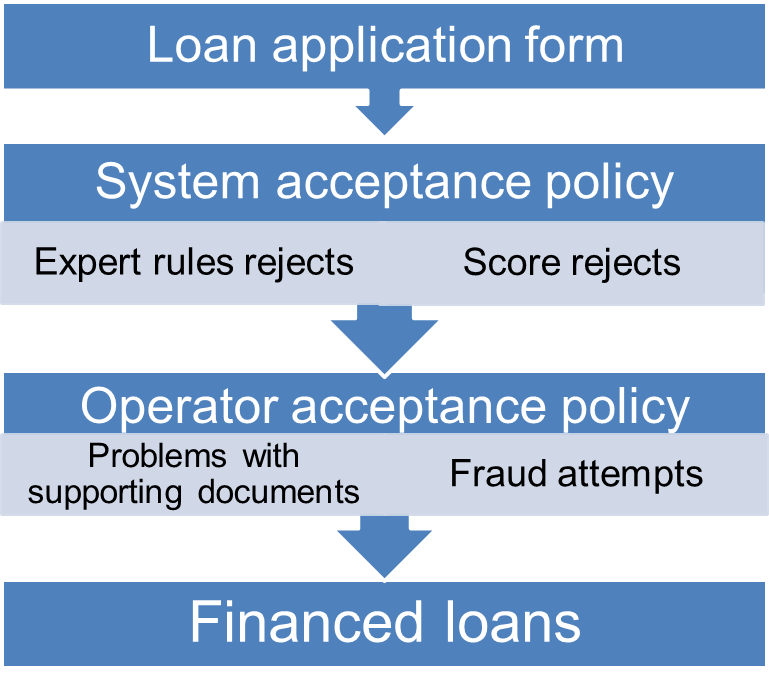
\includegraphics[width=5cm]{figures/chapitre2/schema.png}
\caption{Simplified Acceptance mechanism in~Crédit Agricole Consumer Finance}
\label{fig:figure1}

\end{minipage}%
\hfil \begin{minipage}[b]{0.5\linewidth}

\center 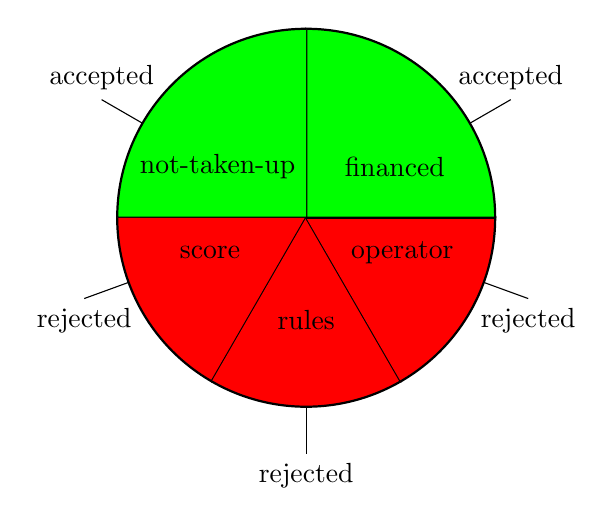
\begin{tikzpicture}

    \foreach \start/\end/\middle/\percent/\anchor/\name in {
      0/90/30/financed/above/accepted,
      90/180/150/not-taken-up/above/accepted}
  {
    \draw[fill=green, thick] (0,0) -- (\end:2.4cm) arc (\end:\start:2.4cm)
      node at (\middle:1.3cm) {\percent};
    \draw (\middle:2.4cm) -- (\middle:3cm) node[\anchor] {\name};
  };
    
    \foreach \start/\end/\middle/\percent/\anchor/\name in {
      180/240/200/score/below/rejected,
      240/300/270/rules/below/rejected,
      300/360/340/operator/below/rejected}
  {
    \draw[fill=red, thick] (0,0) -- (\end:2.4cm) arc (\end:\start:2.4cm)
      node at (\middle:1.3cm) {\percent};
    \draw (\middle:2.4cm) -- (\middle:3cm) node[\anchor] {\name};
  };
\end{tikzpicture}
\caption{Simplified Acceptance status in Crédit Agricole Consumer Finance - scale relations not respected}
\label{fig:figure2}

\end{minipage}
\end{figure}



\begin{figure}[ht]
\center 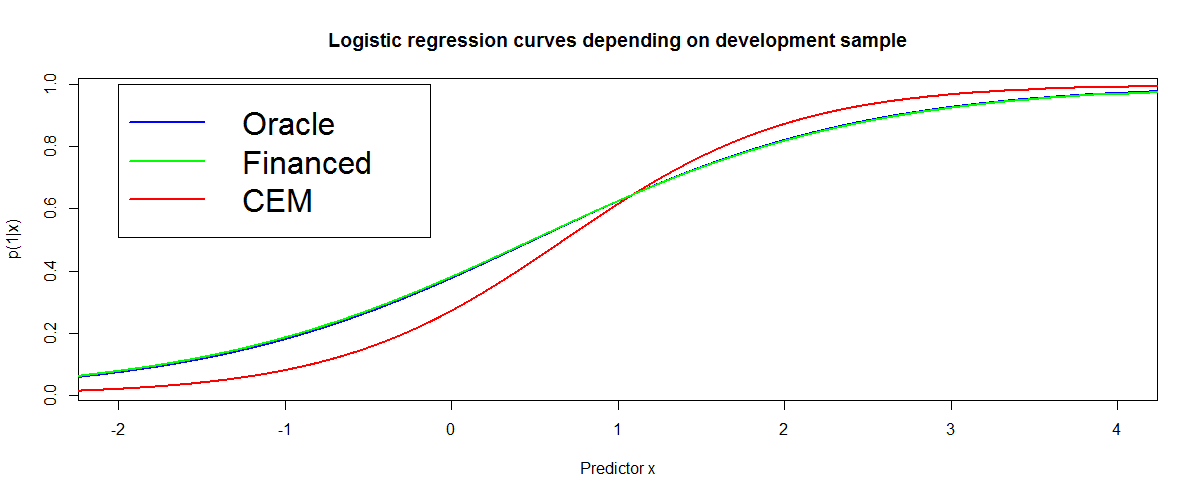
\includegraphics[width=\textwidth]{figures/chapitre2/CEM_bias.png}
\caption{In the context of a probabilistic classifier, it is known that the CEM algorithm employed implicitly by the Reclassification method amounts to a bigger bias in terms of \gls{lr} parameters, but a ``sharper'' decision boundary.}
\label{fig:biais_CEM}
\end{figure}







%\[ \begin{array}{c}
%\tikzmarkin[hor=style green]{el11} \bm{y}^{\text{f}} \tikzmarkend{el11}\\
%\\
%\\
%\tikzmarkin[hor=style orange]{el12} \bm{y}^{\text{nf}} \tikzmarkend{el12}\end{array}
%\left( \begin{array}{c}
%\tikzmarkin[hor=style green]{e4} y_1 \\
%\vdots \\
%y_n \tikzmarkend{e4} \\ 
%\tikzmarkin[hor=style orange]{e3} \text{NA} \\
%\vdots \\
%\text{NA} \tikzmarkend{e3} \end{array} \right) \hspace{1.5cm} \begin{array}{c}
%\tikzmarkin[hor=style green]{el02} \bm{x}^{\text{f}} \tikzmarkend{el02}\\
%\\
%\\
%\tikzmarkin[hor=style orange]{el-12} \bm{x}^{\text{nf}} \tikzmarkend{el-12} \end{array}
%\left( \begin{array}{ccc}
%\rowcolor{red!20}
%\tikzmarkin[hor=style green]{e1} \; \; x_1^1 & \cdots & x_1^d  \\
% \vdots & \vdots & \vdots  \\
% x_n^1 & \cdots & x_n^d \tikzmarkend{e1} \\
%\tikzmarkin[hor=style orange]{e2} \; \; x_{n+1}^1 & \cdots & x_{n+1}^d  \\
% \vdots & \vdots & \vdots \\
% x_{n+m}^1 & \cdots & x_{n+m}^d \tikzmarkend{e2} \end{array} \right)\]





%\[ \begin{array}{c}
%\tikzmarkin[hor=style green]{l1} \bm{y}^{\text{f}} \tikzmarkend{l1}\\
%\\
%\\
%\tikzmarkin[hor=style green]{l2} \bm{y}^{\text{nf}} \tikzmarkend{l2} \end{array}
%\left( \begin{array}{c}
%\tikzmarkin[hor=style green]{l3} \; \; \; \; \; \; \; \; \; \; \; \; \; \; y_1 \; \; \; \; \; \; \; \; \; \; \; \; \; \; \\
%\vdots \\
% y_n \\ 
% p_{\hat{\theta}^{\text{f}}}(Y_{n+1}=1|x_{n+1}) \\
%\vdots \\
%p_{\hat{\theta}^{\text{f}}}(Y_{n+m}=1|x_{n+m}) \tikzmarkend{l3}\end{array} \right) \begin{array}{c}
%\tikzmarkin[hor=style green]{el0} \bm{x}^{\text{f}} \tikzmarkend{el0} \\
%\\
%\\
%\tikzmarkin[hor=style green]{el-1} \bm{x}^{\text{nf}} \tikzmarkend{el-1} \end{array}
%\left( \begin{array}{ccc}
%\rowcolor{red!20}
%\tikzmarkin[hor=style green]{el1} \; \; x_1^1 & \cdots & x_1^d  \\
% \vdots & \vdots & \vdots \\
% x_n^1 & \cdots & x_n^d \\
% x_{n+1}^1 & \cdots & x_{n+1}^d  \\
% \vdots & \vdots & \vdots \\
% x_{n+m}^1 & \cdots & x_{n+m}^d \tikzmarkend{el1} \end{array} \right)\]


\printbibliography[heading=subbibliography, title=References of Chapter 2]